%TCIDATA{Version=5.00.0.2570}
%TCIDATA{LaTeXparent=0,0,Presentation-CAFE-displacement-subdoc.tex}
% $Id: Presentation-JSM-subdoc.tex 398 2013-11-03 22:31:36Z lv39 $
% $URL: https://forge.cornell.edu/svn/repos/ncrn-cornell/branches/papers/JSM2013/Presentation/Presentation-JSM-subdoc.tex $
\section{Introduction}
\begin{frame}{Introduction}
\frametitle{}
\begin{block}{NCRN}
\begin{itemize}
\item This work is part of the NSF Census Research Network (NCRN) - Cornell Node ("Integrated Research Support, Training and Data Documentation")
\item Funded by NSF Grant \href{http://www.nsf.gov/awardsearch/showAward.do?AwardNumber=1131848}{\#1131848}. 
\item For more information, see \href{http://www.ncrn.cornell.edu}{www.ncrn.cornell.edu}.
\end{itemize}
\begin{center}
\href{http://www.ncrn.cornell.edu}{
\includegraphics[width=0.4\textwidth]{qr-ncrn.png}}
\end{center}
\end{block}
\end{frame}

\begin{frame}{Introduction}
\begin{block}{Overview of work}
\begin{itemize}
\item Basic program outlined in Abowd, Vilhuber, and Block (PSD 2012) and Lagoze, Block, Williams, Abowd, and Vilhuber,  International Data Curation Conference (2013)
\item PROV extension described in more detail in Lagoze, Williams, Vilhuber (Metadata and Semantics Research Conference, 2013 - proposed)
\end{itemize}
\end{block}
\end{frame}

%
%
%
\section[Motivation]{Some facts that motivated us}


\begin{frame}
\frametitle{}
\begin{block}{Motivation}

\end{block}
\end{frame}

\begin{frame}
\frametitle{Replication of research results}
\begin{block}{Critical element of science}
\begin{itemize}
\item Replication of methods, data inputs, computational environment is a critical element of the scientific approach
\item Journals, funding agencies (in the U.S.) have been moving to making archiving of inputs to scientific results more robust, even mandatory
\end{itemize}
\end{block}
\end{frame}

\begin{frame}
\frametitle{Not a new problem}
\begin{block}{Econometrica}
``In its first issue, the editor of Econometrica (1933), Ragnar Frisch, noted
the importance of publishing data such that readers could fully explore
empirical results.  Publication of data, however, was discontinued early in
the journal's history.  [...]  The journal arrived full-circle in late 2004 when Econometrica
adopted one of the more stringent policies on availability of data and
programs.
\end{block}
\tiny \href{http://www.econometricsociety.org/submissions.asp\#4}{http://www.econometricsociety.org/submissions.asp\#4} as cited in \href{http://research.stlouisfed.org/wp/2005/2005-014.pdf}{Anderson et al (2005)}
\end{frame}

\begin{frame}
\frametitle{Problem will become worse}
\begin{block}{Increased use of restricted-access data}
\begin{itemize}
\item Today's young scholars pursue research
programs that mandate inherently identifiable data
\begin{itemize}
\item Geospatial relations,
\item Exact genome data,
\item Networks of all sorts,
\item Linked administrative records
\end{itemize}
\item These researchers acquire authorized, generally unfettered, restricted access to the
confidential, identifiable data and perform their analyses in secure
environments.
\item Archiving (curation) of input data is complicated
\item Knowledge discovery is complicated
\end{itemize}
\end{block}
\end{frame}
\begin{frame}
\frametitle{Decline in the use of classic public-use data}
%\includepdf[pages={1-2}]{Chetty-1-2-Slides.pdf}
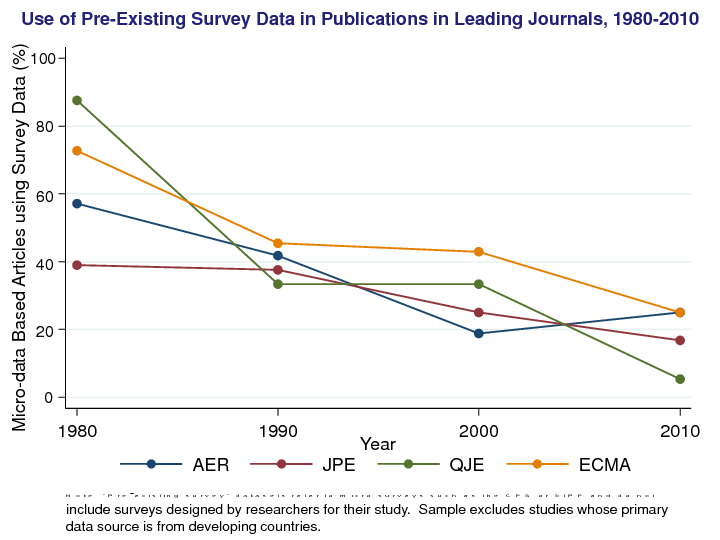
\includegraphics[width=0.7\paperwidth]{ChettySlide1}
\end{frame}

\begin{frame}
\frametitle{Increase in the use of administrative data in economics}
%\includepdf[pages={1-2}]{Chetty-1-2-Slides.pdf}
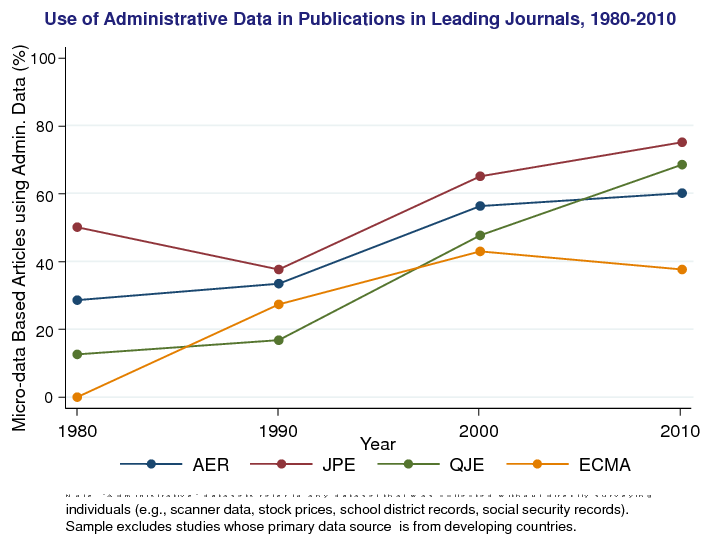
\includegraphics[width=0.7\paperwidth]{ChettySlide2}
\end{frame}

\begin{frame}
\frametitle{Not limited to economics}
\begin{block}{Nature, 2012}
``Many of the emerging `big data' applications come from private sources that are inaccessible to other researchers. The data source may be hidden, compounding problems of verification, as well as concerns about the generality of the results.''\\
\end{block}
{\tiny (Huberman, Nature 482, 308 (16 February 2012) \href{http://dx.doi.org/10.1038/482308d}{doi:10.1038/482308d})}
\begin{block}{Other domains}
\begin{itemize}
\item Biology (genetics data, chemical compounds)
\item Computer science (search records, single-firm examples)
\end{itemize}
\end{block}
\end{frame}

\section[Problem]{Stating the problem in the U.S. case}
%\begin{frame}
%\frametitle{}
%\begin{block}{Stating the problem}
%
%\end{block}
%\end{frame}

\begin{frame}
\frametitle{Why we think there is a problem}
\begin{block}{Core issues}
\begin{itemize}
\item[a] Insufficient curation (starting with archiving)
\item[b] No way to reference data (unique identifiers)
\item[c] No consistent way to learn about the data (metadata dissemination)
\item[d] Weak or non-existent provenance tracing
\end{itemize}
\end{block}
\end{frame}

\begin{frame}{Generalized problem}
\begin{block}{Multiple data sources in the US}
\begin{itemize}
\item U.S. Census Bureau (RDC) \hyperlink{Census}{\beamergotobutton{more}}
\item Internal Revenue Service (confidential, public-use)\hyperlink{IRS}{\beamergotobutton{more}}
\item Bureau of Labor Statistics (confidential, public-use data)\hyperlink{BLS}{\beamergotobutton{more}}

\end{itemize}
\end{block}
\begin{block}{Present elsewhere?}
\begin{itemize}
\item Canada: 
\begin{itemize}
\item Centre for Data Development and Economic Research (CDER: RDC-like for business data)\hyperlink{CDER}{\beamergotobutton{more}}
\item better: Canadian RDC network\hyperlink{CRDC}{\beamergotobutton{more}}
\end{itemize}
\item France: better: R\'eseau Quetelet\hyperlink{France}{\beamergotobutton{more}}
\item Germany?
\end{itemize}
\end{block}
\end{frame}


%\begin{frame}
%\frametitle{Core problems}
%\begin{columns}
%  \begin{column}{0.3\textwidth}
%    \begin{itemize}[<+->]
%\item Curation\newline
%\item Identification\newline
%\item Information dissemination
%    \end{itemize}
%  \end{column}
%  \begin{column}{0.25\textwidth}
%  \begin{itemize}
%  \item[\ ]\onslide<4-6>{$\leftarrow$}\newline
%  \item[\ ]\onslide<5-6>{$\leftarrow$}\newline
%  \item[\ ]\onslide<6>{$\leftarrow$}\newline
%  \end{itemize}
%  \end{column}
%  \begin{column}{0.4\textwidth}
%     \begin{itemize}[<+->]
%        \item require cooperation of NSI
%        \item partial solution (DOI)\newline
%        \item core proposal\newline
%     \end{itemize}
%  \end{column}
%\end{columns}
%\end{frame}


\section[Solution]{A proposed solution}
\begin{frame}
\frametitle{}
\begin{block}{CED$^2$AR: A proposed solution}

\end{block}
\end{frame}

\begin{frame}
\frametitle{Comprehensive Extensible Data Documentation and Access (CED$^2$AR)}
\begin{block}{Core}
We develop the core of a method for solving the data archive
and curation problem that confronts the custodians of restricted-access
research data and the scientific users of such data. Our solution recognizes 
the dual protections afforded by physical security and access limitation protocols.
\end{block}
\end{frame}

\begin{frame}
\frametitle{Requirements}
\begin{block}{Royal Society (2012)}
\begin{itemize}
\item Accessible (a researcher can easily find it);
\item Intelligible (to various audiences);
\item Assessable (are researchers able make judgements about or
assess the quality of the data);
\item Usable (at minimum, by other scientists).
\end{itemize}
\end{block}
\end{frame}


\begin{frame}
\frametitle{Proposed solution}
\begin{block}{Extensible framework}
\begin{itemize}[<+->]
\item Based on existing standards (\href{http://www.ddialliance.org}{Data Documentation Initiative}, DDI) with extension to accomodate disclosure protection mechanisms
\item Connectors (import/export) to other sources and standards
\item To be filled by multiple sources of metadata (some the curators/owners, others ``crowd-sourced'')
\item Interim solution for those datasets without unique identifiers (\href{http://datacite.org/whatisdoi}{Digital Object Identifier}, DOI)
\end{itemize}
\end{block}
\end{frame}


%\begin{frame}
%\frametitle{Extensions to DDI}
%\begin{block}{Basic idea}
%\begin{tabular}{rcl}
%\only<1>{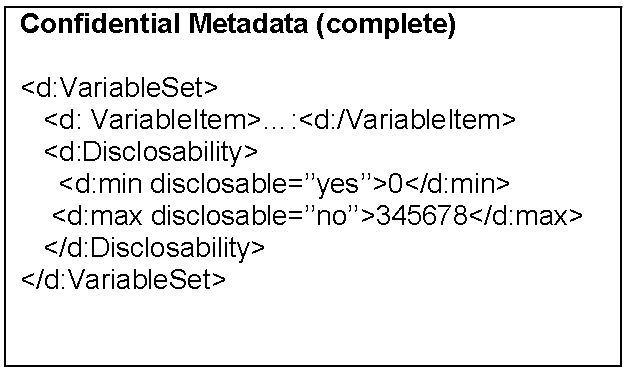
\includegraphics[width=0.4\textwidth]{ConfidentialMetadata-left}}
%\only<2->{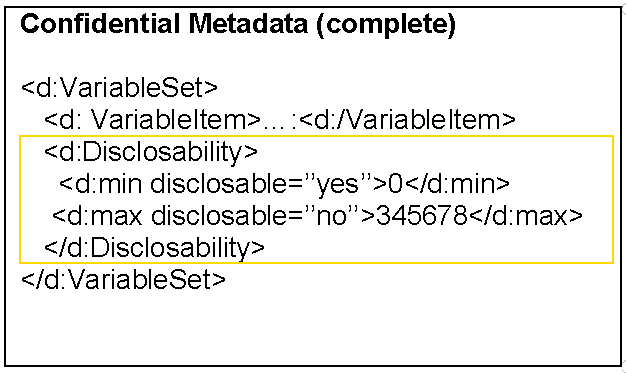
\includegraphics[width=0.4\textwidth]{ConfidentialMetadata-left-hilite}}\pause \pause &
%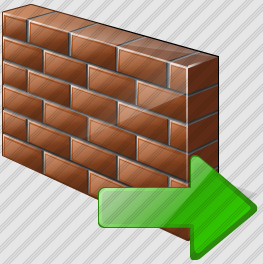
\includegraphics[width=0.1\textwidth]{wall-export-small}&
%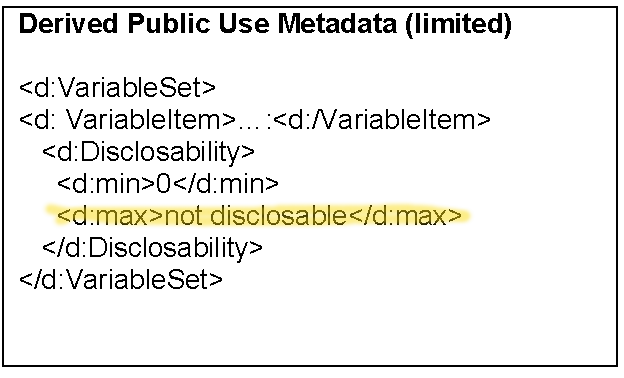
\includegraphics[width=0.4\textwidth]{ConfidentialMetadata-right}
%\end{tabular}
%\end{block}
%\end{frame}

\begin{frame}
\frametitle{Database design}
\begin{block}{Multiple sources}
\begin{itemize}
\item Data-curator-provided metadata (possibly regularly updated, PRUNED)
\item Alternate sources (IPUMS data to describe Decennial Census)
\item {\bf User-provided metadata (wiki) (planned fall 2013)}
\end{itemize}
\end{block}
\begin{block}{Multiple outputs}
\begin{itemize}
\item Local query ({\bf working})
\item Remote federation or export
\item Synchronization back to data-curator (data enclave!)
\end{itemize}
\end{block}
\end{frame}

\begin{frame}{Provenance}
\begin{block}{The provenance problem}
``data provenance, one kind of metadata, pertains to the derivation history of a
data product starting from its original sources'' [...]  ``from it, one can ascertain
the quality of the data base and its ancestral data and derivations, track back sources
of errors, allow automated reenactment of derivations to update the data, and provide 
attribution of data sources'' 
\end{block}
{\tiny Simmhan, Plale, and Gannon, ``A survey of data provenance in e-science,'' ACM Sigmod Record, 2005}
\end{frame}


\begin{frame}{Provenance (cont)}
\begin{block}{PROV model}
W3C PROV Model  based in the notions of 
\begin{enumerate}
\item \textbf{entities} that are physical, digital, and conceptual
things in the world; 
\item \textbf{activities} that are dynamic aspects of the world that change and
create entities; and 
\item \textbf{agents} that are responsible for activities. 
\item  a set of \textbf{relationships} that can exist be-
tween them that express attribution,. delegation, derivation, etc.
\end{enumerate}
\end{block}
\begin{block}{PROV and Metadata}
Not (currently) a ``native'' component of DDI
\end{block}
\end{frame}

\begin{frame}{Incorporating PROV (LBD)}
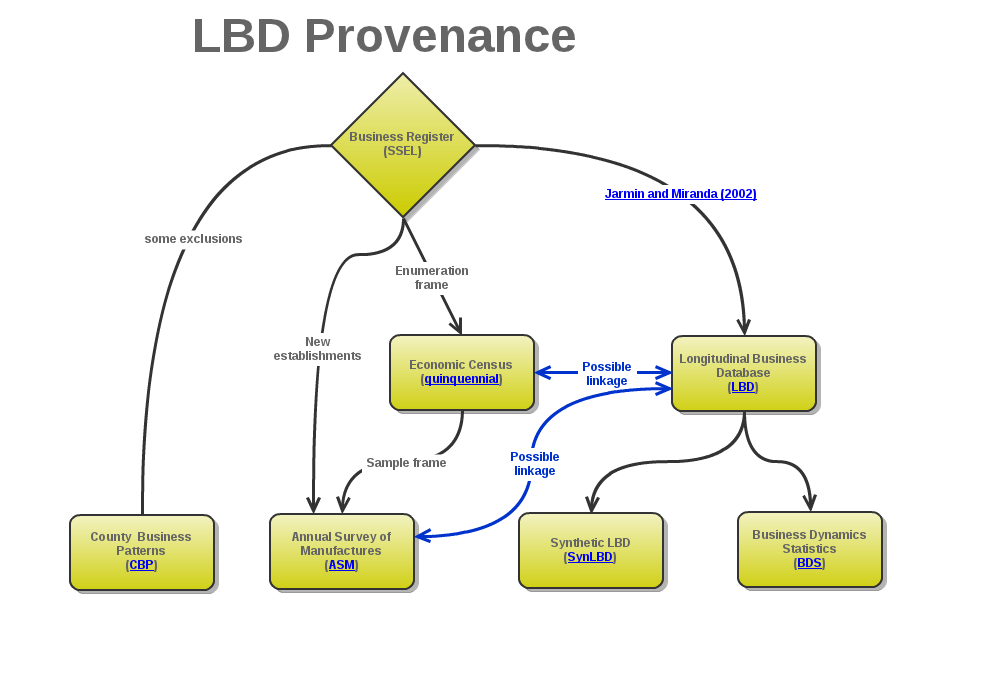
\includegraphics[width=\textwidth]{LBD_Provenance.png}
\end{frame}

\begin{frame}{Incorporating PROV (LBD)}
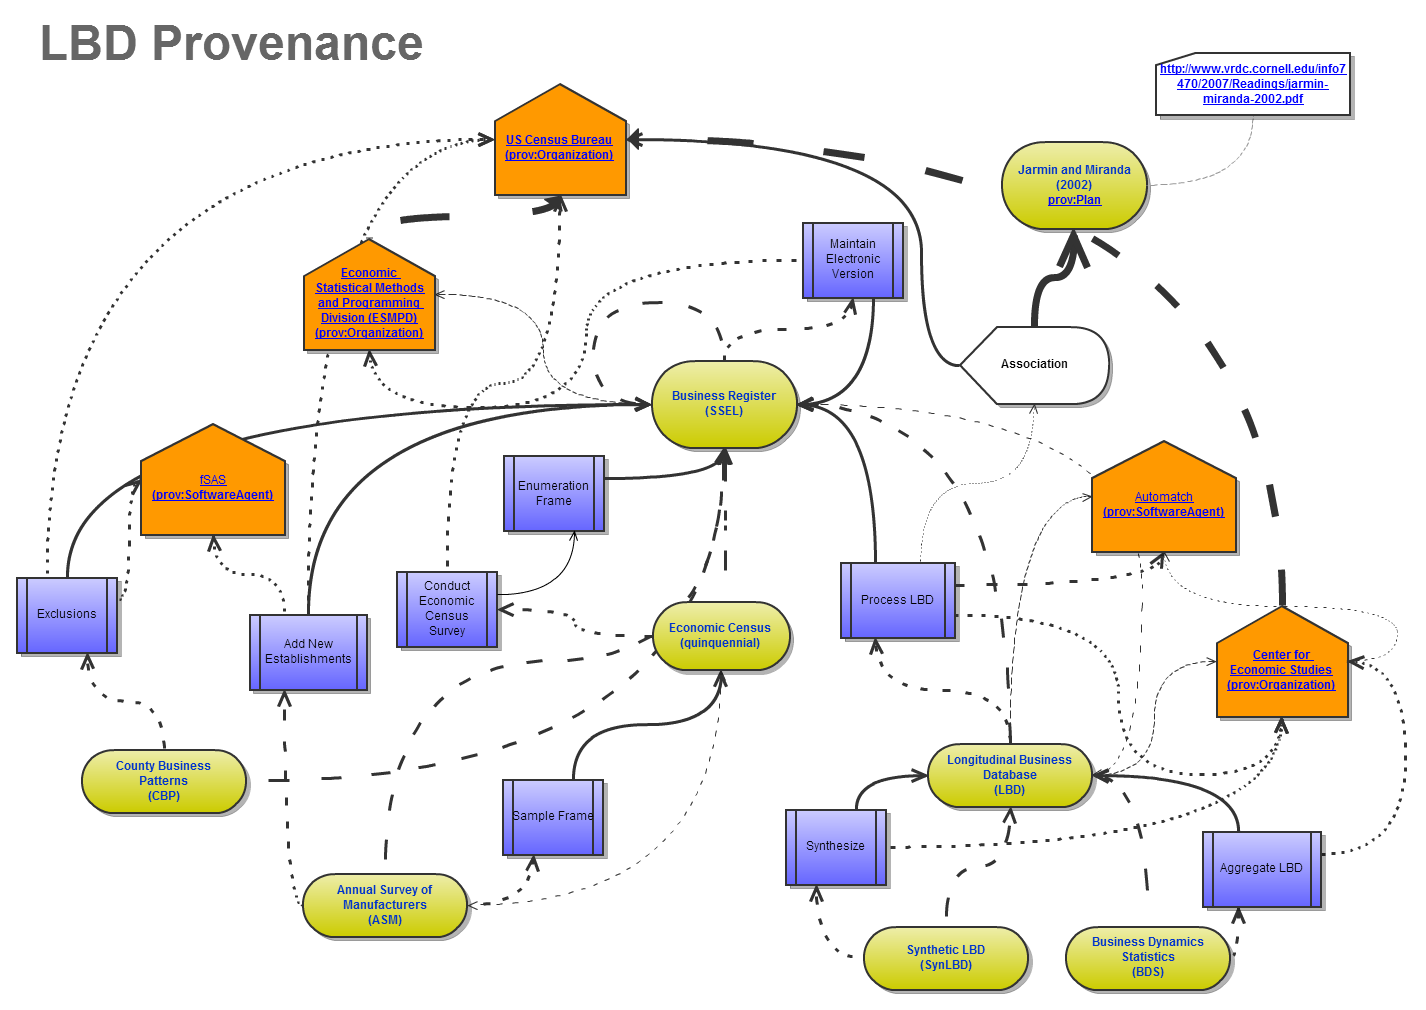
\includegraphics[width=0.9\textwidth]{LBD_PROV_-_WIP.png}
\end{frame}

\begin{frame}{Incorporating PROV (LBD)}
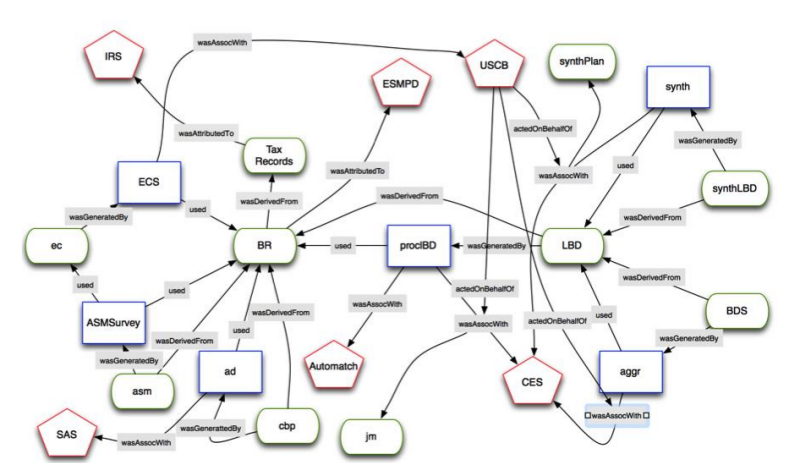
\includegraphics[width=0.9\textwidth]{LBD_Prov_simplified.png}
\end{frame}

\begin{frame}{Incorporating PROV (LBD)}
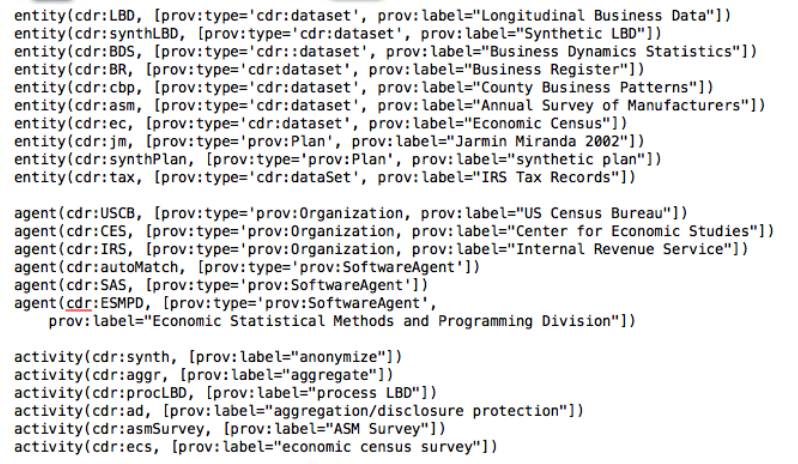
\includegraphics[width=0.9\textwidth]{LBD_Prov_simplified_text.png}
\end{frame}

\begin{frame}{Work on PROV}
\begin{block}{More details forthcoming}
See Lagoze, Williams, Vilhuber ``Encoding Provenance Metadata for
Social Science Datasets'', submitted to Metadata and Semantics Research Conference (soon)
\end{block}
\end{frame}

%\begin{frame}
%\frametitle{Generic description}
%\centering
%\includegraphics[width=0.9\textwidth]{"CCBMR"}
%\end{frame}
%
%\begin{frame}[fragile]
%\frametitle{Identifiers}
%\begin{block}{Unique identifiers for {\it articles}}
%\begin{verbatim}
%Huberman, B. A.
%Sociology of science:
%Big data deserve a bigger audience
%Nature, 2012, 482, 308-308
%doi:10.1038/482308d
%\end{verbatim}
%\end{block}
%\begin{block}{Unique identifiers for {\it data}}
%``DOI names are assigned to any entity for use on digital networks. 
%They are used to provide current information, including where they (or information about them) can be found on the Internet.
%Information about a digital object may change over time, including where to find it, but its DOI name will not change.''
%\tiny http://datacite.org/whatisdoi, accessed on Sept 26, 2012.
%\end{block}
% \end{frame}

\begin{frame}
\frametitle{State of the implementation}
\begin{block}{DDI extension}
Being incorporated.
\end{block}
\begin{block}{DOI assignment}
Our project (NCRN) will assign/register DOI if not provided by curator/owner
\end{block}
\begin{block}{Database}
Design finalized, database populated with  metadata for newest SIPP Synthetic Beta. Wiki additions  Fall 2013
\end{block}
\begin{block}{UI}
Version 1.1 of the UI being completed (more robust, scalable). Wiki additions in Fall 2013
\end{block}
\begin{block}{Provenance}
PROV extension, integration Winter 2013/14
\end{block}

\end{frame}

\begin{frame}{Screenshot}
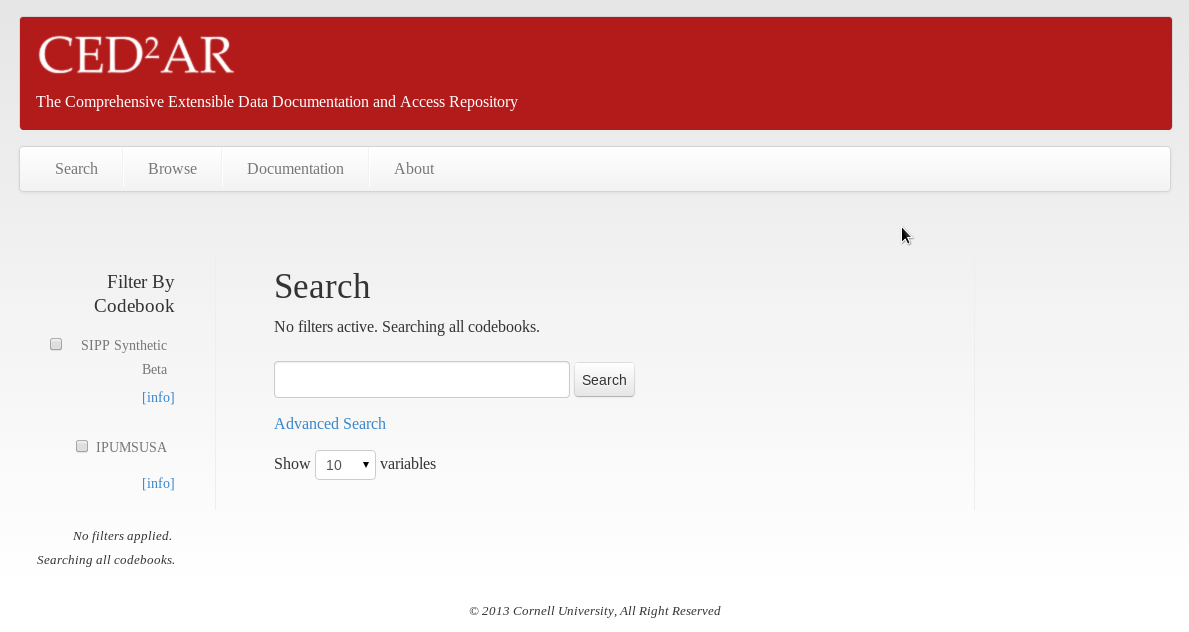
\includegraphics[width=\textwidth]{ced2ar-20130803.png}
\end{frame}

\begin{frame}{Screenshot}
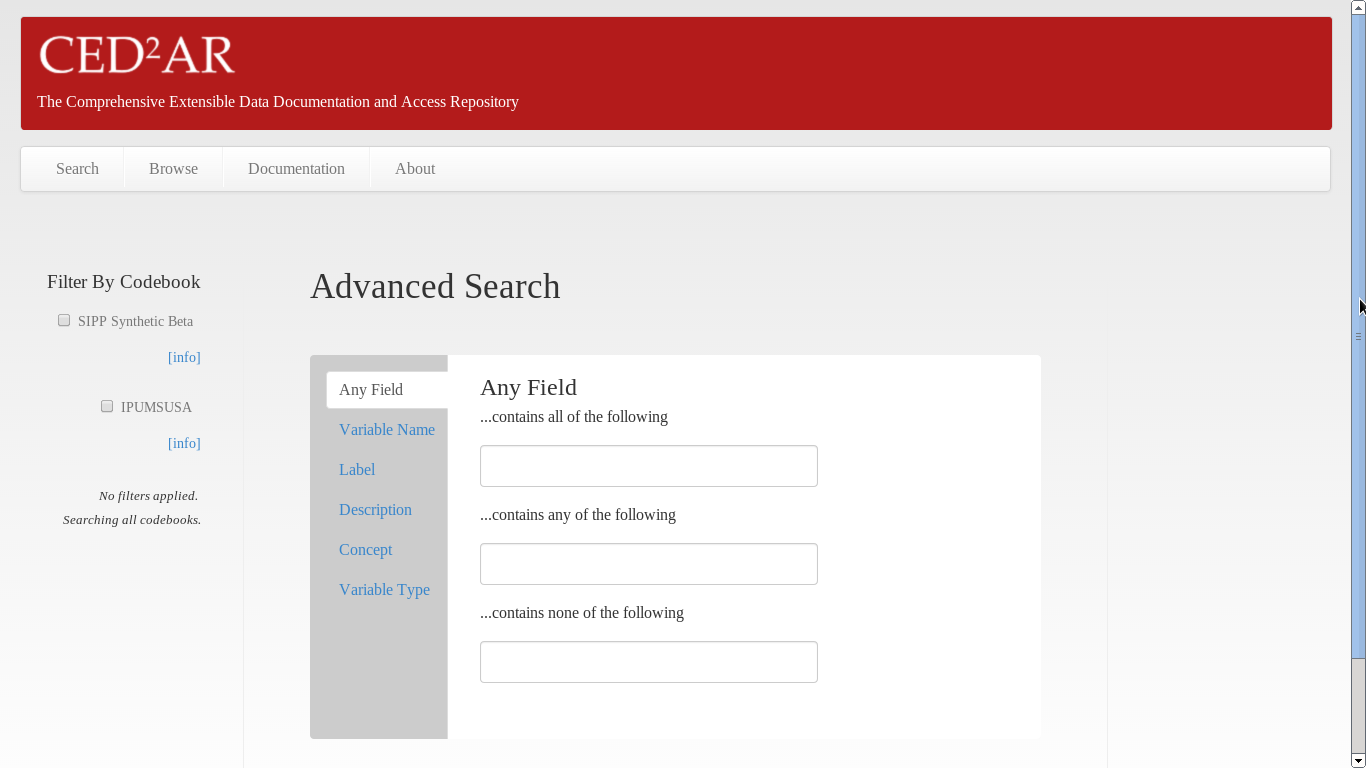
\includegraphics[width=\textwidth]{ced2ar-20130803-advanced.png}
\end{frame}
\begin{frame}{Screenshot}
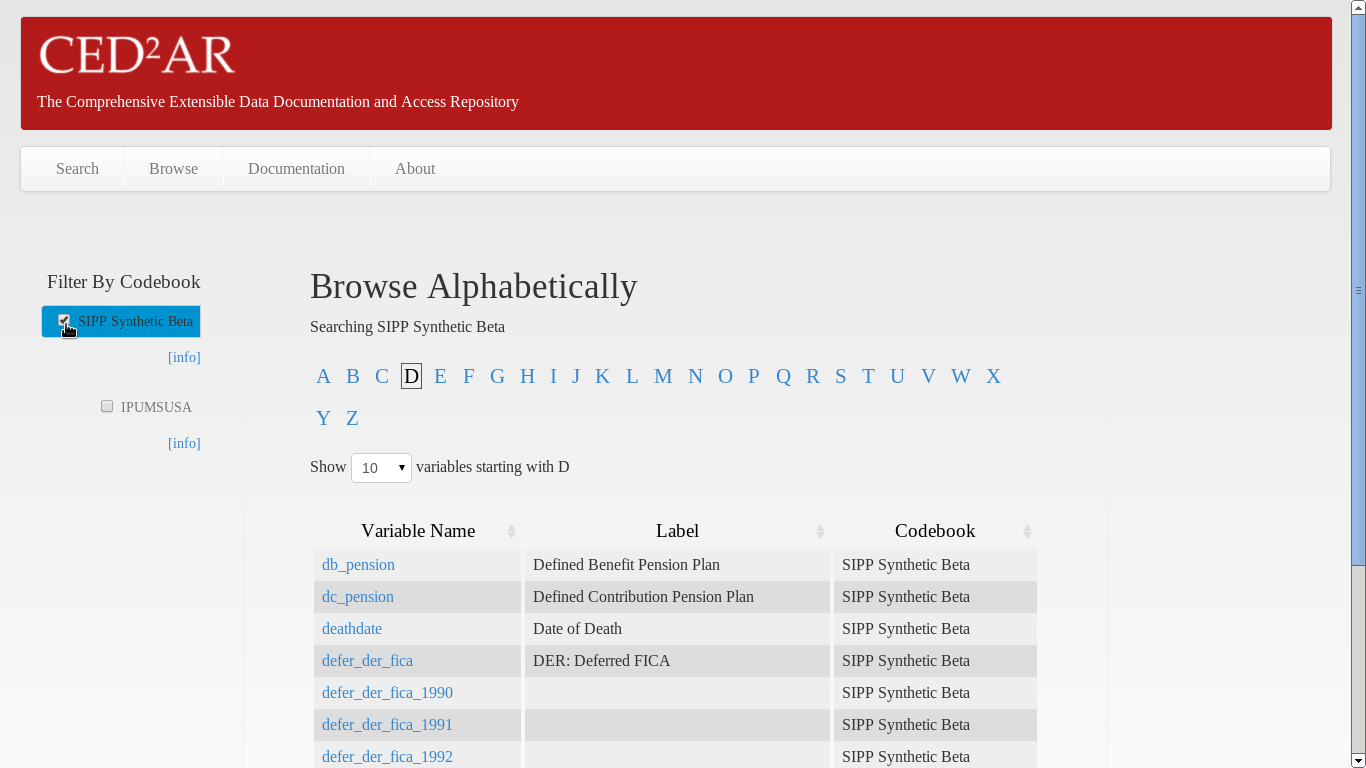
\includegraphics[width=\textwidth]{ced2ar-20130803-browse.png}
\end{frame}

\subsection{Further links}
\begin{slide}
\frametitle{The end}
\begin{block}{Thank you}
\begin{itemize}
\item \cite{AbowdVilhuberBlock2012} for more details
\item \href{http://www.ilr.cornell.edu/LDI/}{Labor Dynamics Institute}
\item \href{http://www.vrdc.cornell.edu}{VirtualRDC @ Cornell}
\item \href{http://www.ncrn.cornell.edu/}{NCRN Cornell website}
\end{itemize}
\end{block}
\end{slide}

\begin{frame}[fragile]
\begin{verbatim}
$Id: Presentation-JSM-subdoc.tex 398 2013-11-03 22:31:36Z lv39 $
\end{verbatim}
\end{frame}

%%% Local Variables:
%%% mode: latex
%%% End:
